\chapter{Simulation of birth-death tree and TDA detection}

There are two directions under this project. Since they both rely on the simulation of a stochastic birth-death tree, they are grouped here together.

The pseudo-code for the simulation of the birth-death tree is shown below:
\section{Simulation of the birth-death tree}
\begin{algorithm}[H]
\caption{Birth--Death--Hybridization (BDH) simulation}
\begin{algorithmic}[1]
\State Initialize $G$ with root and $1$--$2$ starting leaves; $t \gets 0$
\While{$|\mathcal{L}| > 0$ and $|\mathcal{L}| < N_{\text{stop}}$}
    \State $n \gets |\mathcal{L}|$
    \State $r_{\text{spec}} \gets n\lambda$,\quad $r_{\text{ext}} \gets n\mu$,\quad $r_{\text{hyb}} \gets \binom{n}{2}\nu$
    \State $r_{\text{tot}} \gets r_{\text{spec}} + r_{\text{ext}} + r_{\text{hyb}}$
    \State draw $\Delta t \sim \text{Exp}(r_{\text{tot}})$; \quad $t \gets t + \Delta t$
    \If{$t \geq \text{age}$}
        \State $t \gets \text{age}$; \textbf{break}
    \EndIf
    \State sample $u \in \mathcal{L}$ uniformly; draw $\rho \sim \text{Unif}(0,1)$
    \If{$\rho < r_{\text{spec}} / r_{\text{tot}}$}
        \State \textsc{Speciate}$(u)$ \Comment{$u \to$ two new leaves}
    \ElsIf{$\rho < (r_{\text{spec}} + r_{\text{ext}}) / r_{\text{tot}}$}
        \State \textsc{Extinguish}$(u)$ \Comment{mark $u$ extinct, remove from $\mathcal{L}$}
    \Else
        \State sample $v \in \mathcal{L} \setminus \{u\}$; draw inheritance $\iota \sim \pi_{\text{inher}}$
        \State draw event type $\in \{\text{generating}, \text{degenerative}, \text{neutral}\}$ w.p. $\propto$ \textsc{hybprops}
        \State \textsc{Hybridize}$(u, v, \iota, \text{type})$ \Comment{merge lineages, add reticulation edge(s)}
    \EndIf
\EndWhile
\State seal all pendant edges to current leaves
\State \Return $G$
\end{algorithmic}
\end{algorithm}

\section{Detection of reticulation edge in the simulated trees}

Once the tree is produced, it needs to be populated to accurately capture its topology. 

\subsection{Lit review}
NeighborNet:

\cite{feged2026shape,bryant2004neighbor}

\subsection{State of the project}
Across 24 simulations, cycle detection tracked the largest reticulation-induced distance shortening in the dressed tip–tip matrix. All 21 simulations with a cycle had a maximum shortening $\geq52\%$, while the three with no cycle had only $22–36\%$, with no overlap (point-biserial correlation -0.86); when reticulation edges do not meaningfully shorten any tip-to-tip path, no distance-space hole exists to recover, so the missing cycles reflect genuine signal loss rather than detection failure. This held only after removing the Rips-filtration cap, which had suppressed valid cycles in sim18 and sim23. 

A separate limitation is the recovery criterion itself: requiring both endpoints of a cycle edge to be leaves currently discards 4 hybrid detections (sim6, sim7, sim12) in which the hybrid lies on a nonzero-weight cycle edge paired with an internal node; relaxing the rule to "hybrid on any nonzero-weight cycle edge" restores these without affecting the remaining genuinely uncaptured hybrids.

\begin{table}[htbp]
  \centering
  \caption{Inheritance-weight asymmetry of reticulation edges recovered versus
    missed by the cycle-closing edge. Here \texttt{inher\_weight} is the
    minor-parent inheritance proportion, bounded to $(0,0.5]$, so distance from
    $0.5$ measures hybridization asymmetry. Pooled over 24 simulations.}
  \label{tab:inher-weight-recovery}
  \begin{tabular}{lcccc}
    \toprule
    & $n$ & mean \texttt{inher\_weight} & mean $|\texttt{inher}-0.5|$ & median $|\texttt{inher}-0.5|$ \\
    \midrule
    Found & 33 & 0.371 & 0.129 & 0.103 \\
    Missed                         & 98 & 0.200 & 0.300 & 0.313 \\
    \bottomrule
  \end{tabular}
\end{table}
Missed reticulation edges are far more asymmetric than recovered ones
(Table~\ref{tab:inher-weight-recovery}): since \texttt{inher\_weight} is bounded above by $0.5$, ``far from $0.5$'' means a near-negligible minor parent. Of the $99$ missed edges, $32$ have $\texttt{inher\_weight} < 0.1$, versus $1$ of $32$ recovered edges. This follows from the model: the reticulate path has length $\texttt{primary\_inher}\cdot d_{12}$, so when the minor parent contributes little the hybrid sits on its major parent, the shortcut is weak, and the tip-distance metric acquires no hole. It mirrors the $-0.86$ correlation between cycle detection and dressing-induced distance shortening, with \texttt{inher\_weight} as the causal parameter.

But this method can detect higher dimensional reticulate edges

--actually, more than one shortest paths can be used

\section{Detection of reticulation edges in the union of gene trees}
The previous section produces a network with reticulate edges present. In this section, we produce a set of gene trees based on the reticulated network and attempt to detect the reticulate edges in the union of the gene trees. 

Different from the previous project, the gene trees do not need to be populated because there are only edges of weight 1.

To illustrate the full pipeline, we use a small toy network throughout this section, built to match \texttt{sim\_bdh.py}'s \texttt{hyb\_generating} mechanics exactly (the only hybridization type this project's simulations actually use). The reticulation node $H$ has in-degree 2, receiving an edge from both $A$ and $B$ --- both edges are present simultaneously in the network as simulated, before any filtering or gene-tree resolution takes place. Critically, \texttt{hyb\_generating} gives \emph{each} parent its own continuation leaf ($A_3$ for $A$, $D$ for $B$) in addition to its edge into $H$ --- neither parent's identity depends on which side of the reticulation is later resolved:

\begin{figure}[h]
\centering
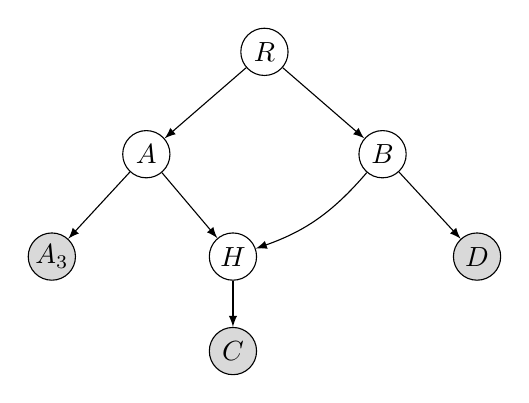
\begin{tikzpicture}[
    leaf/.style={circle,draw,fill=gray!30,minimum size=6mm,inner sep=0pt},
    internal/.style={circle,draw,fill=white,minimum size=6mm,inner sep=0pt}
]
\node[internal] (R)  at (0,0)        {$R$};
\node[internal] (A)  at (-1.5,-1.3)  {$A$};
\node[internal] (B)  at (1.5,-1.3)   {$B$};
\node[leaf]     (A3) at (-2.7,-2.6)  {$A_3$};
\node[internal] (H)  at (-0.4,-2.6)  {$H$};
\node[leaf]     (D)  at (2.7,-2.6)   {$D$};
\node[leaf]     (C)  at (-0.4,-3.8)  {$C$};

\draw[-latex] (R) -- (A);
\draw[-latex] (R) -- (B);
\draw[-latex] (A) -- (A3);
\draw[-latex] (A) -- (H);
\draw[-latex] (B) -- (D);
\draw[-latex] (B) to[bend left=15] (H);
\draw[-latex] (H) -- (C);
\end{tikzpicture}
\caption{The original simulated network: 7 nodes, one reticulation. $H$ has in-degree 2, fed by both $A\!\to\!H$ and $B\!\to\!H$; $A$ and $B$ each also keep their own continuation leaf ($A_3$, $D$) regardless of which retic edge later survives. This is the network gene tree 1 and gene tree 2 (below) are each a single resolution of.}
\end{figure}

For each network, we decompose the network into a set of gene trees (as shown below). We first filter the network so that it no longer has hybrid nodes and extinct nodes. Then we enumerate the output to the set of gene trees, each of which takes a specific combination of all gene selections. We show two examples of the gene trees which differ because of their different choices in the event of hybridisation. During enumeration, we remove any dead ends (hanging nodes that were not labelled $"is\_leaf"$) iteratively and we remove any nodes with only one out-going nodes.
\begin{figure}[h]
\centering
\begin{minipage}{0.48\textwidth}
\centering
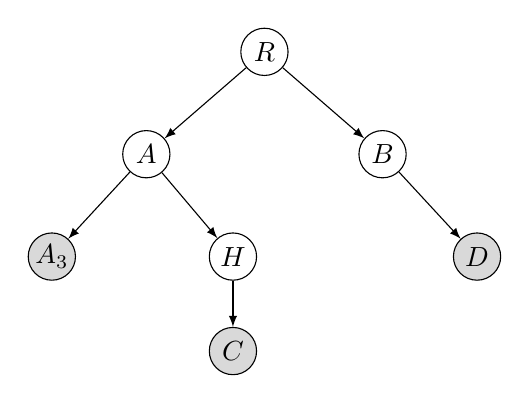
\begin{tikzpicture}[
    leaf/.style={circle,draw,fill=gray!30,minimum size=6mm,inner sep=0pt},
    internal/.style={circle,draw,fill=white,minimum size=6mm,inner sep=0pt}
]
\node[internal] (R)  at (0,0)        {$R$};
\node[internal] (A)  at (-1.5,-1.3)  {$A$};
\node[internal] (B)  at (1.5,-1.3)   {$B$};
\node[leaf]     (A3) at (-2.7,-2.6)  {$A_3$};
\node[internal] (H)  at (-0.4,-2.6)  {$H$};
\node[leaf]     (D)  at (2.7,-2.6)   {$D$};
\node[leaf]     (C)  at (-0.4,-3.8)  {$C$};

\draw[-latex] (R) -- (A);
\draw[-latex] (R) -- (B);
\draw[-latex] (A) -- (A3);
\draw[-latex] (A) -- (H);
\draw[-latex] (B) -- (D);
\draw[-latex] (H) -- (C);
\end{tikzpicture}

\small Gene tree 1: $A\!\to\!H$ retained, $B\!\to\!H$ dropped --- $A$ stays a genuine 2-child branch ($A_3$, $H$); $B$ is now unary (only $D$ left) and will suppress away
\end{minipage}
\hfill
\begin{minipage}{0.48\textwidth}
\centering
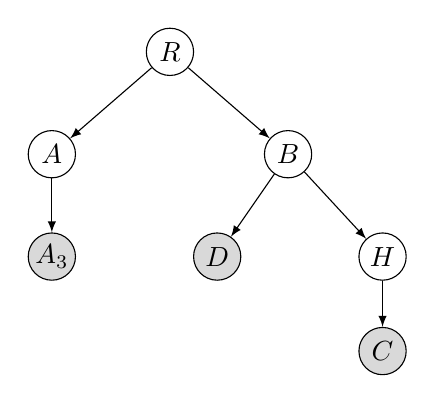
\begin{tikzpicture}[
    leaf/.style={circle,draw,fill=gray!30,minimum size=6mm,inner sep=0pt},
    internal/.style={circle,draw,fill=white,minimum size=6mm,inner sep=0pt}
]
\node[internal] (R)  at (0,0)        {$R$};
\node[internal] (A)  at (-1.5,-1.3)  {$A$};
\node[internal] (B)  at (1.5,-1.3)   {$B$};
\node[leaf]     (A3) at (-1.5,-2.6)  {$A_3$};
\node[leaf]     (D)  at (0.6,-2.6)   {$D$};
\node[internal] (H)  at (2.7,-2.6)   {$H$};
\node[leaf]     (C)  at (2.7,-3.8)   {$C$};

\draw[-latex] (R) -- (A);
\draw[-latex] (R) -- (B);
\draw[-latex] (A) -- (A3);
\draw[-latex] (B) -- (D);
\draw[-latex] (B) -- (H);
\draw[-latex] (H) -- (C);
\end{tikzpicture}

\small Gene tree 2: $B\!\to\!H$ retained, $A\!\to\!H$ dropped --- $B$ stays a genuine 2-child branch ($D$, $H$); $A$ is now unary (only $A_3$ left) and will suppress away
\end{minipage}
\caption{Two gene-tree resolutions of the same 7-node network, differing by which edge into the reticulate node $H$ is kept. Gray nodes are leaves, white nodes are internal. $H$ itself is unary in both resolutions (its only child is always $C$), so it suppresses away regardless of which parent feeds it.}
\end{figure}

\begin{figure}[h]
\centering
\begin{minipage}{0.48\textwidth}
\centering
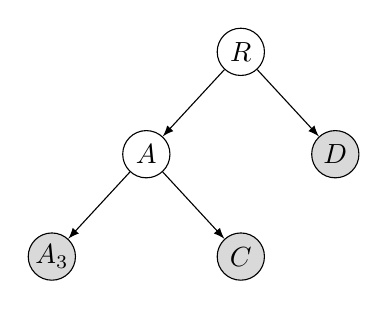
\begin{tikzpicture}[
    leaf/.style={circle,draw,fill=gray!30,minimum size=6mm,inner sep=0pt},
    internal/.style={circle,draw,fill=white,minimum size=6mm,inner sep=0pt}
]
\node[internal] (R)  at (0,0)       {$R$};
\node[internal] (A)  at (-1.2,-1.3) {$A$};
\node[leaf]     (D)  at (1.2,-1.3)  {$D$};
\node[leaf]     (A3) at (-2.4,-2.6) {$A_3$};
\node[leaf]     (C)  at (0,-2.6)    {$C$};

\draw[-latex] (R) -- (A);
\draw[-latex] (R) -- (D);
\draw[-latex] (A) -- (A3);
\draw[-latex] (A) -- (C);
\end{tikzpicture}

\small Gene tree 1 (suppressed): $B$ and $H$ both had exactly one outgoing edge, so they contract away in sequence --- $R\!\to\!B\!\to\!D$ collapses to $R\!\to\!D$, and $A\!\to\!H\!\to\!C$ collapses to $A\!\to\!C$
\end{minipage}
\hfill
\begin{minipage}{0.48\textwidth}
\centering
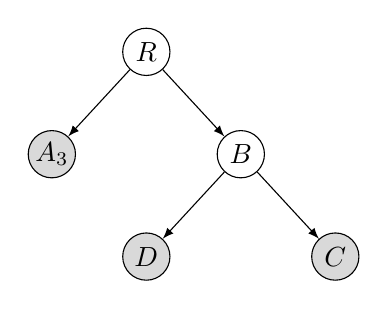
\begin{tikzpicture}[
    leaf/.style={circle,draw,fill=gray!30,minimum size=6mm,inner sep=0pt},
    internal/.style={circle,draw,fill=white,minimum size=6mm,inner sep=0pt}
]
\node[internal] (R)  at (0,0)       {$R$};
\node[leaf]     (A3) at (-1.2,-1.3) {$A_3$};
\node[internal] (B)  at (1.2,-1.3)  {$B$};
\node[leaf]     (D)  at (0,-2.6)    {$D$};
\node[leaf]     (C)  at (2.4,-2.6)  {$C$};

\draw[-latex] (R) -- (A3);
\draw[-latex] (R) -- (B);
\draw[-latex] (B) -- (D);
\draw[-latex] (B) -- (C);
\end{tikzpicture}

\small Gene tree 2 (suppressed): $A$ and $H$ both had exactly one outgoing edge, so they contract away in sequence --- $R\!\to\!A\!\to\!A_3$ collapses to $R\!\to\!A_3$, and $B\!\to\!H\!\to\!C$ collapses to $B\!\to\!C$
\end{minipage}
\caption{The two gene trees from the previous figure after iteratively removing every node with only one outgoing edge. $H$ disappears in both trees; additionally $B$ disappears in tree 1 and $A$ disappears in tree 2 --- whichever parent lost its edge into $H$ is the one left unary and suppressed. Both resulting trees keep all four leaves $\{A_3, D, C\}$ plus whichever of $A$/$B$ survived as a branch point.}
\end{figure}

After the gene trees are generated, we start labelling them using unions of leaves.

\begin{figure}[h]
\centering
\begin{minipage}{0.48\textwidth}
\centering
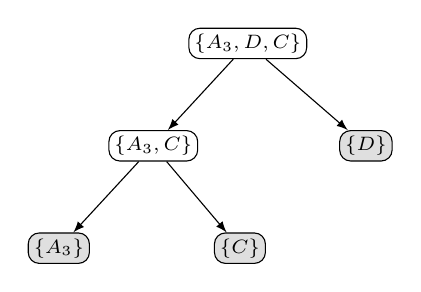
\begin{tikzpicture}[
    leaf/.style={draw,rounded corners,fill=gray!25,inner sep=2pt,font=\scriptsize},
    internal/.style={draw,rounded corners,fill=white,inner sep=2pt,font=\scriptsize}
]
\node[internal] (R)  at (0,0)       {$\{A_3,D,C\}$};
\node[internal] (A)  at (-1.2,-1.3) {$\{A_3,C\}$};
\node[leaf]     (D)  at (1.5,-1.3)  {$\{D\}$};
\node[leaf]     (A3) at (-2.4,-2.6) {$\{A_3\}$};
\node[leaf]     (C)  at (-0.1,-2.6) {$\{C\}$};

\draw[-latex] (R) -- (A);
\draw[-latex] (R) -- (D);
\draw[-latex] (A) -- (A3);
\draw[-latex] (A) -- (C);
\end{tikzpicture}

\small Gene tree 1
\end{minipage}
\hfill
\begin{minipage}{0.48\textwidth}
\centering
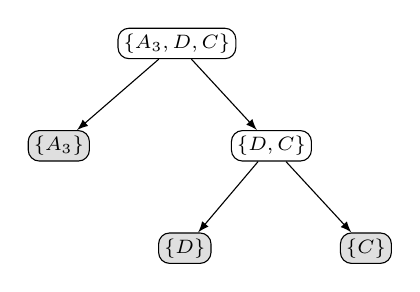
\begin{tikzpicture}[
    leaf/.style={draw,rounded corners,fill=gray!25,inner sep=2pt,font=\scriptsize},
    internal/.style={draw,rounded corners,fill=white,inner sep=2pt,font=\scriptsize}
]
\node[internal] (R)  at (0,0)       {$\{A_3,D,C\}$};
\node[leaf]     (A3) at (-1.5,-1.3) {$\{A_3\}$};
\node[internal] (B)  at (1.2,-1.3)  {$\{D,C\}$};
\node[leaf]     (D)  at (0.1,-2.6)  {$\{D\}$};
\node[leaf]     (C)  at (2.4,-2.6)  {$\{C\}$};

\draw[-latex] (R) -- (A3);
\draw[-latex] (R) -- (B);
\draw[-latex] (B) -- (D);
\draw[-latex] (B) -- (C);
\end{tikzpicture}

\small Gene tree 2
\end{minipage}
\caption{Both gene trees relabelled by the union of leaves under each node, in preparation for merging them into one graph. Note $R$'s label is now \emph{identical} in both trees ($\{A_3,D,C\}$, the leaf set every \texttt{hyb\_generating} resolution shares) --- unlike a network where the two resolutions' leaf sets genuinely differ, agreement here is guaranteed by construction.}
\end{figure}

\texttt{tree\_addition.py} merges two trees by identifying nodes with identical leaf-set labels. Here $R$, $A_3$, $D$, and $C$ all match across the two relabelled trees above --- every leaf agrees, and so does the root, since both trees cover the same total leaf set. Only $A=\{A_3,C\}$ (tree 1) and $B=\{D,C\}$ (tree 2) stay distinct, since their descendant sets differ depending on which parent survived as a branch point. Merging on this many shared points closes more than one cycle:

\begin{figure}[h]
\centering
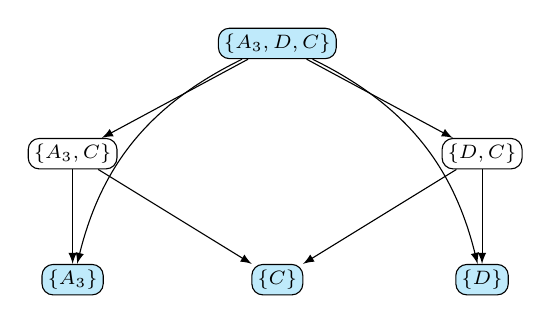
\begin{tikzpicture}[
    leaf/.style={draw,rounded corners,fill=gray!25,inner sep=2pt,font=\scriptsize},
    internal/.style={draw,rounded corners,fill=white,inner sep=2pt,font=\scriptsize},
    shared/.style={draw,rounded corners,fill=cyan!25,inner sep=2pt,font=\scriptsize}
]
\node[shared]   (R)  at (0,1.4)      {$\{A_3,D,C\}$};
\node[internal] (A)  at (-2.6,0)     {$\{A_3,C\}$};
\node[internal] (B)  at (2.6,0)      {$\{D,C\}$};
\node[shared]   (A3) at (-2.6,-1.6)  {$\{A_3\}$};
\node[shared]   (C)  at (0,-1.6)     {$\{C\}$};
\node[shared]   (D)  at (2.6,-1.6)   {$\{D\}$};

\draw[-latex] (R) -- (A);
\draw[-latex] (R) -- (B);
\draw[-latex] (A) -- (A3);
\draw[-latex] (A) -- (C);
\draw[-latex] (B) -- (D);
\draw[-latex] (B) -- (C);
\draw[-latex] (R) to[bend right=25] (A3);
\draw[-latex] (R) to[bend left=25] (D);
\end{tikzpicture}
\caption{Merging gene tree 1 and gene tree 2 by leaf-set identity. The shared nodes $\{A_3,D,C\}$, $\{A_3\}$, $\{D\}$, $\{C\}$ (cyan) are where the two trees' own edges ($R\!\to\!A_3$ from tree 1's suppression, $R\!\to\!D$ from tree 2's) land directly on the other tree's already-shared nodes, while $\{A_3,C\}$ and $\{D,C\}$ stay tree-specific. This 6-node, 8-edge graph has $E-V+1=3$ independent cycles: two triangles ($R$--$A$--$A_3$ and $R$--$B$--$D$) plus one 4-cycle ($R$--$A$--$C$--$B$). Unlike the earlier (leaf-set-inconsistent) version of this example, an accurate single-reticulation \texttt{hyb\_generating} network does not collapse to one clean cycle --- each parent's own leaf independently closes its own small loop with the (now-shared) root, on top of the main loop through the shared hybrid leaf $C$. \texttt{find\_cycles.py} must recover the reticulation signal from among all three.}
\end{figure}

\section{To dos}
Find a mapping between the nodes and their parent so perhaps we can recover the edge information from these node sets

randomly generate gene trees: simulate several times and build a distribution and the new method (picture see phone)

1. prove: 1/2 threshold
2. largest harmonic edge is also the closing edge. 

Look into Mapper

!!!:

check: if the reticulate edge can walk in the directed graph to A or B, then the shortest path can be defined on the undirected graph with that reticulate edge, otherwise, delete that reticulate edge and then walk:
in def $_build_output(state: SimState)$: change the how the distance is defined. and also tip to tip i assume. 



